\usetikzlibrary{arrows.meta}

\begin{frame}{too much milk: is it possible}
\begin{itemize}
\item is there a solutions with writing/reading notes?
    \begin{itemize}
    \item $\approx$ loading/storing from shared memory
    \end{itemize}
\vspace{.5cm}
\item yes, but it's not very elegant
\end{itemize}
\end{frame}

\begin{frame}[fragile,label=solutionFour]{too much milk: solution 4 (algorithm)}
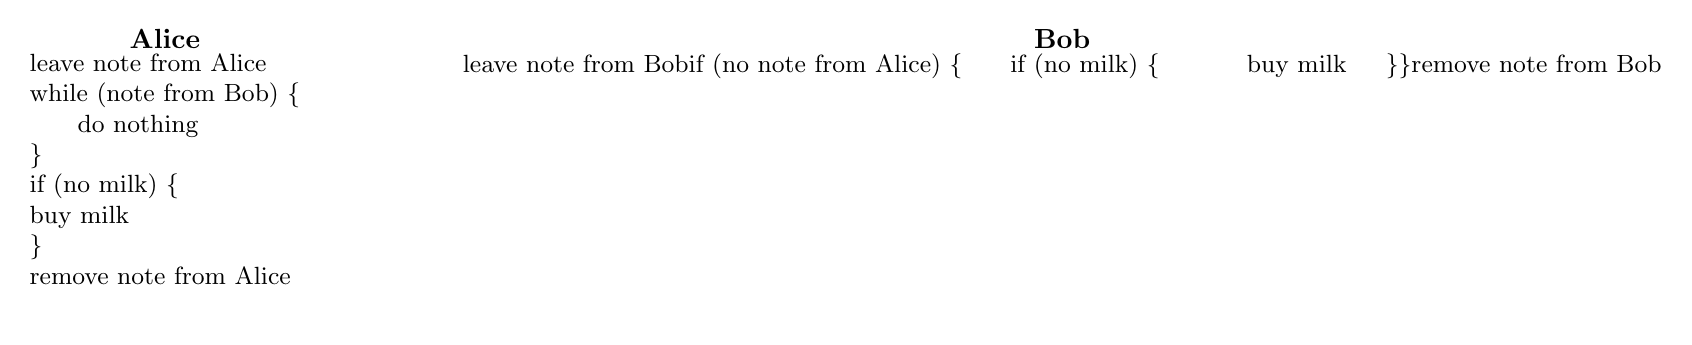
\begin{tikzpicture}
\tikzset{
    >=Latex,
}
\begin{scope}
\tikzset{
    every label/.style={font=\bfseries},
    every node/.style={inner sep=0.25mm,font=\small},
}
\node[label={north:Alice},align=left,anchor=north west] (thread A part 1) {
leave note from Alice \\
while (note from Bob) \{ \\
\hspace{0.5cm} do nothing \\
\} \\
if (no milk) \{ \\
    buy milk \\
\} \\
remove note from Alice \\
};
\node[label={north:Bob},anchor=north west] (thread B part 1) at ([xshift=2cm]thread A part 1.north east) {
leave note from Bob \\
if (no note from Alice) \{ \\
\hspace{0.5cm} if (no milk) \{ \\
\hspace{1cm} buy milk \\
\hspace{0.5cm}\} \\
\} \\
remove note from Bob \\
};
\end{scope}
\end{tikzpicture}
\begin{itemize}
\item<2-> exercise (hard): prove (in)correctness
\item<4-> exercise (hard): extend to three people
\end{itemize}
\end{frame}

\begin{frame}{Peterson's algorithm}
    \begin{itemize}
        \item general version of solution
        \item see, e.g., Wikipedia
            \vspace{.5cm}
        \item we'll use special hardware support instead
    \end{itemize}
\end{frame}
